%-------------------------------------------------------------------------------
\section{Results}
\label{sec:result}
%-------------------------------------------------------------------------------

This section presents the results obtained from the individual channel, as well as their combination,
following the statistical analysis discussed in Section~\ref{sec:stat_analysis}.

A binned likelihood fit under the signal-plus-background hypothesis is performed on the BDT discriminant distributions in the four 
analysis regions considered. The unconstrained parameters of the fit are the signal 
strength, and four independent parameters associated with the normalisation of the fake $\had$ background in each of the analysis regions. 
No significant pulls or constraints are obtained for the fitted nuisance parameters, resulting in a post-fit background prediction in each analysis region that is
very close to the pre-fit prediction, albeit with reduced uncertainties due to the anti-correlations among sources of systematic uncertainty resulting from the fit.
Figure~\ref{fig:asimov_prefitbdt} shows a comparison of the data and prediction for the BDT discriminant distribution in
the search channels. Figure~\ref{fig:asimov_postfitbdtHc} and~\ref{fig:asimov_postfitbdtHu} show a post-fit to the asimov data for the $tHc$ and $tHu$ search separately.
%both pre- and post-fit to data, in the case of the $\Hc$ search.  
%A similar comparison for the leptonic channel is shown in Figure~\ref{fig:tthML_trexPrefit} and \ref{fig:tthML_trexPrefit_1}.
Tables summarising the pre-fit and post-fit yields can be found in Appendix~\ref{sec:prepostfit_yields_Htautau_appendix}.


%\input{\FCNCFigures/tex/tthML_trexPrefit}
%\input{\FCNCFigures/tex/xTFW_trexPrefit}
\begin{figure}[H]
\centering
\includegraphics[width=0.33\textwidth]{\FCNCFigures/tthML/Limit/tcH_reg1l2tau1bnj_os_postFit.pdf}
\put(-30, 110){\small\textbf{(a1)}}
\includegraphics[width=0.33\textwidth]{\FCNCFigures/tthML/Limit/tcH_reg1l1tau1b1j_ss_postFit.pdf}
\put(-30, 110){\small\textbf{(a2)}}
\includegraphics[width=0.33\textwidth]{\FCNCFigures/tthML/Limit/tcH_reg1l1tau1b2j_ss_postFit.pdf}
\put(-30, 110){\small\textbf{(a3)}}\\
\includegraphics[width=0.33\textwidth]{\FCNCFigures/tthML/Limit/tcH_reg1l1tau1b2j_os_postFit.pdf}
\put(-30, 110){\small\textbf{(b1)}}
\includegraphics[width=0.33\textwidth]{\FCNCFigures/tthML/Limit/tcH_reg1l1tau1b3j_os_postFit.pdf}
\put(-30, 110){\small\textbf{(b2)}}\\
\includegraphics[width=0.33\textwidth]{\FCNCFigures/xTFW/Limit/tcH_reg2mtau1b2jos_vetobtagwp70_highmet_postFit.pdf}
\put(-30, 110){\small\textbf{(c1)}}
\includegraphics[width=0.33\textwidth]{\FCNCFigures/xTFW/Limit/tcH_reg2mtau1b3jos_vetobtagwp70_highmet_postFit.pdf}
\put(-30, 110){\small\textbf{(c2)}}\\
\caption{ The BDT output distributions are fitted to the asimov data in $tHc$ search: $t_l\thadhad$ (a1),  $t_l\tauhad$-1j (a2),  $t_l\tauhad$-2j (a3),
  $t_h\tlhad$-2j (b1), $t_h\tlhad$-3j (b2), $t_h\thadhad$-2j (c1), and $t_h\thadhad$-3j (c2). }
\label{fig:asimov_postfitbdtHc}
\end{figure}

\begin{figure}[H]
\centering
\includegraphics[width=0.33\textwidth]{\FCNCFigures/tthML/Limit/tuH_reg1l2tau1bnj_os_postFit.pdf}
\put(-30, 110){\small\textbf{(a1)}}
\includegraphics[width=0.33\textwidth]{\FCNCFigures/tthML/Limit/tuH_reg1l1tau1b1j_ss_postFit.pdf}
\put(-30, 110){\small\textbf{(a2)}}
\includegraphics[width=0.33\textwidth]{\FCNCFigures/tthML/Limit/tuH_reg1l1tau1b2j_ss_postFit.pdf}
\put(-30, 110){\small\textbf{(a3)}}\\
\includegraphics[width=0.33\textwidth]{\FCNCFigures/tthML/Limit/tuH_reg1l1tau1b2j_os_postFit.pdf}
\put(-30, 110){\small\textbf{(b1)}}
\includegraphics[width=0.33\textwidth]{\FCNCFigures/tthML/Limit/tuH_reg1l1tau1b3j_os_postFit.pdf}
\put(-30, 110){\small\textbf{(b2)}}\\
\includegraphics[width=0.33\textwidth]{\FCNCFigures/xTFW/Limit/tuH_reg2mtau1b2jos_vetobtagwp70_highmet_postFit.pdf}
\put(-30, 110){\small\textbf{(c1)}}
\includegraphics[width=0.33\textwidth]{\FCNCFigures/xTFW/Limit/tuH_reg2mtau1b3jos_vetobtagwp70_highmet_postFit.pdf}
\put(-30, 110){\small\textbf{(c2)}}\\
\caption{ The BDT output distributions are fitted to the asimov data in $tHu$ search: $t_l\thadhad$ (a1),  $t_l\tauhad$-1j (a2),  $t_l\tauhad$-2j (a3),
  $t_h\tlhad$-2j (b1), $t_h\tlhad$-3j (b2), $t_h\thadhad$-2j (c1), and $t_h\thadhad$-3j (c2). }
\label{fig:asimov_postfitbdtHu}
\end{figure}


%Comparison between the data and prediction for the BDT discriminant distribution in the
%$\lephad$ channel, before and after the fit to data  (``Pre-Fit'' and ``Post-Fit'', respectively) under the signal-plus-background hypothesis.
%Shown are the ($\lephad$, 3j) region (a) pre-fit and (c) post-fit, and the ($\lephad$, $\geq$4j) region (b) pre-fit and (d) post-fit.
%The contributions with real $\had$ candidates from $\ttbar$,  $\ttbar V$, $\ttbar H$, and single-top-quark backgrounds are combined into
%a single background source referred to as ``Top (real $\had$)'', whereas the small contributions from 
%$Z\to \ell^+\ell^-$ ($\ell = e, \mu$) and diboson backgrounds are combined into ``Other''. 
%In the pre-fit figures the expected $\Hc$ signal (solid red) corresponding to $\BR(t\to Hc)=1\%$ is also shown,
%added to the background prediction. In the post-fit figures, the $\Hc$ signal is normalised using the best-fit branching ratio, 
%$\BR(t\to Hc)=(-4.4^{+9.9}_{-8.5})\times 10^{-4}$.
%The bottom panels display the ratios of data to either the SM background prediction before the fit (``Bkg'')  or the total signal-plus-background
%prediction after the fit (``Pred''). 
%The hashed area represents the total uncertainty of the background. 
%In the case of the pre-fit background uncertainty, the normalisation uncertainty of the fake $\had$ background is not included.


The best-fit branching ratio obtained is $\BR(t\to Hc)=[-4.4^{+7.7}_{-7.0}\,(\mathrm{stat})^{+6.2}_{-4.9}\,(\mathrm{syst})] \times 10^{-4}$, assuming $\BR(t\to Hu)=0$. 
The best-fit normalisation factors for the fake $\had$ background are: $0.82 \pm 0.23$ in the ($\lephad$, 3j) region, $0.84^{+0.25}_{-0.28}$ in the ($\lephad$, $\geq$4j) region,
$0.94^{+0.18}_{-0.17}$ in the ($\hadhad$, 3j) region, and $0.90 \pm 0.26$ in the ($\hadhad$, $\geq$4j) region.
A similar fit is performed for the $\Hu$ search, yielding $\BR(t\to Hu)=[-5.3^{+7.3}_{-6.5}\,(\mathrm{stat})^{+5.3}_{-4.2}\,(\mathrm{syst})] \times 10^{-4}$,
assuming $\BR(t\to Hc)=0$. The obtained normalisation factors for the fake $\had$ background agree within 1\% with those obtained by the $\Hc$ search.
In both cases, the uncertainty of the measured branching ratio is dominated by the statistical uncertainty.
The main contributions to the total systematic uncertainty arise from the fake $\had$ background estimation and the uncertainty associated
with the different responses to quark-initiated and gluon-initiated jets. 
No significant excess of data events above the background expectation is found, 
and observed (expected) 95\% CL limits are set on $\BR(t\to Hc)$ and $\BR(t\to Hu)$:
$\BR(t\to Hc)<1.9 \times 10^{-3}\,(2.1 \times 10^{-3})$ and $\BR(t\to Hu)<1.7 \times 10^{-3}\,(2.0 \times 10^{-3})$.
These results are dominated by the $\hadhad$ channel, which has a sensitivity a factor of two better than that of the $\lephad$ channel.

\begin{figure*}[t!]
\begin{center}
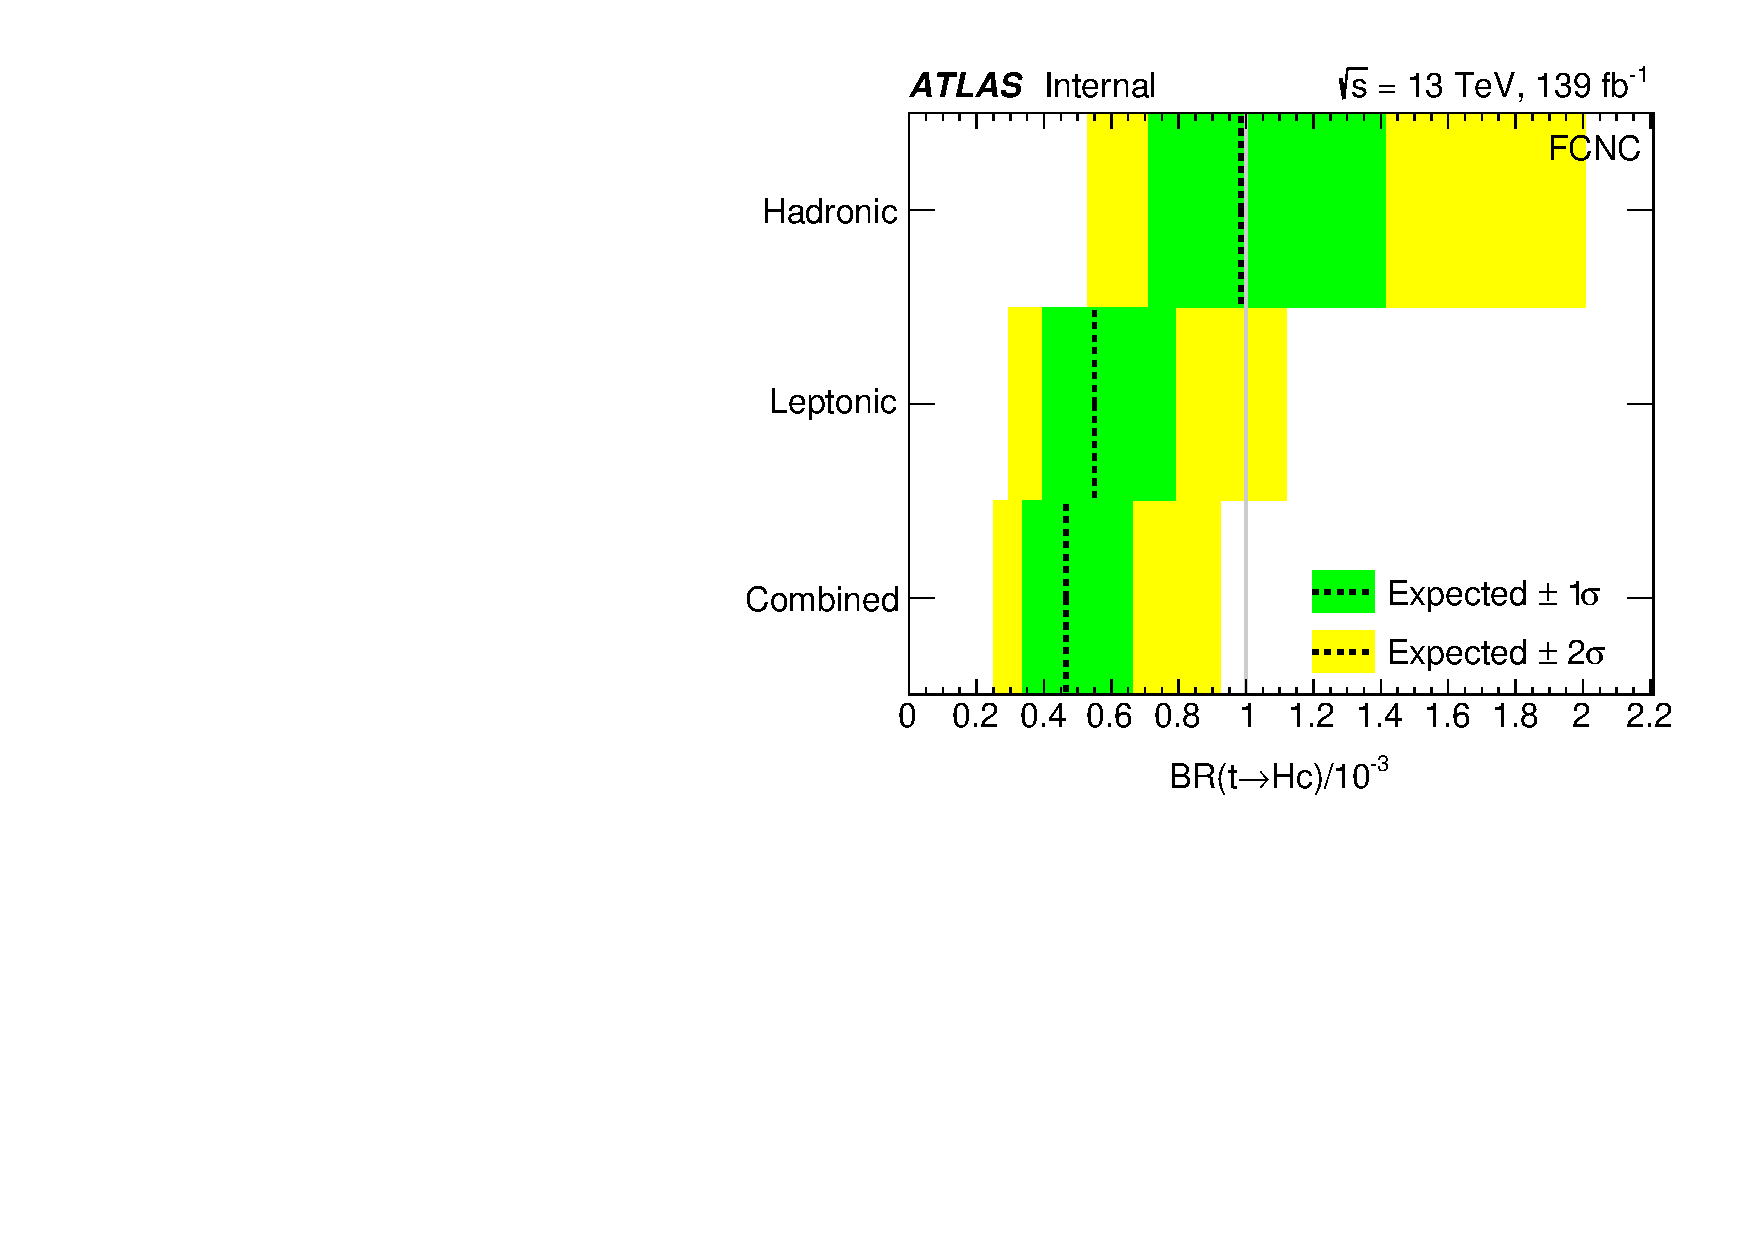
\includegraphics[width=0.7\textwidth]{\FCNCFigures/tcH_combined_Limit.pdf}
\caption{\small {Summary of the best-fit $\BR(t\to Hc)$ for the individual channels as well as their combination,
assuming $\BR(t\to Hu)=0$. (TBD: updated with best fit plots.)}}
\label{fig:summary_printnum_hc} 
\end{center}
\end{figure*}
%%%%%%%%%%%%%%
%%%%%%%%%%%%%%
\begin{figure*}[h!]
\begin{center}
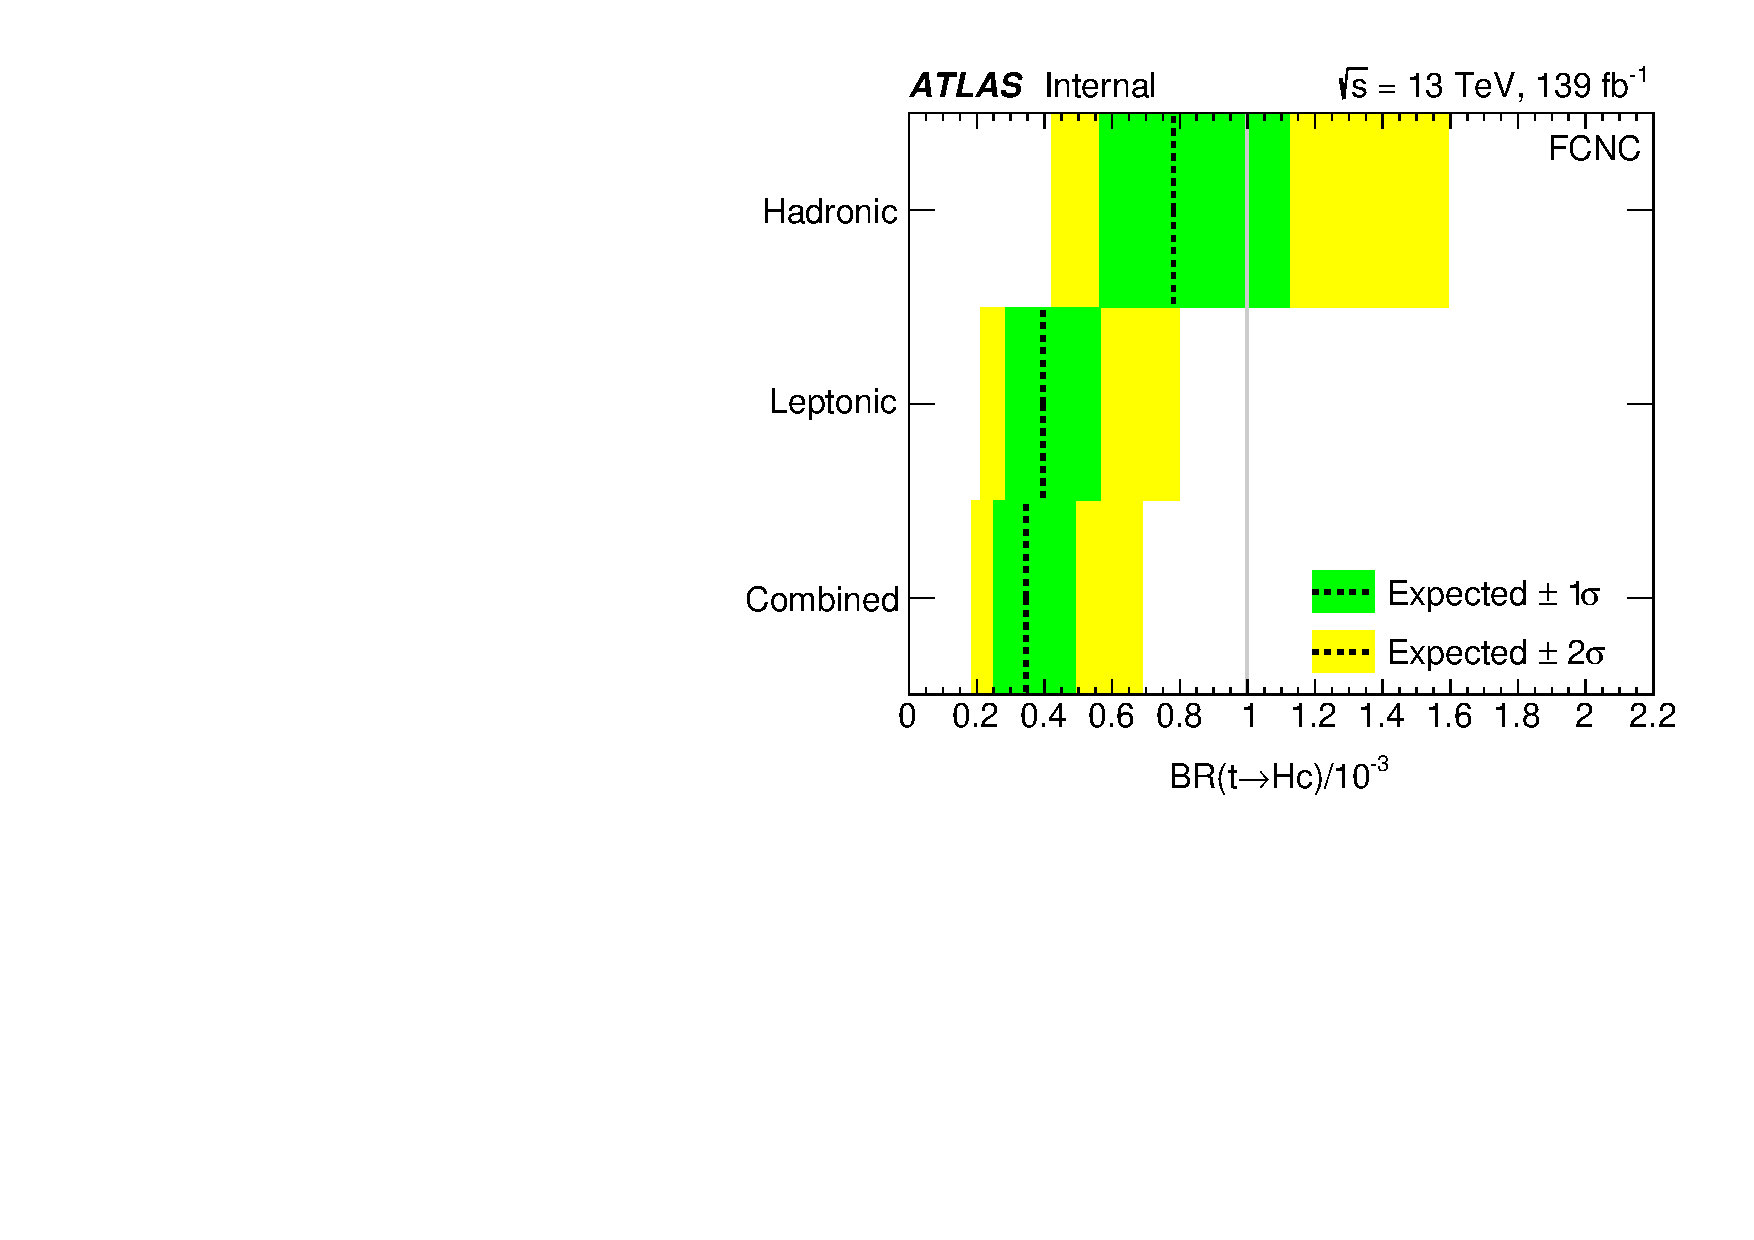
\includegraphics[width=0.7\textwidth]{\FCNCFigures/tuH_combined_Limit.pdf}
\caption{\small {Summary of the best-fit $\BR(t\to Hu)$ for the individual channels as well as their combination,
assuming $\BR(t\to Hc)=0$. (TBD: updated with best fit plots.)}}
\label{fig:summary_printnum_hu} 
\end{center}
\end{figure*}
%%%%%%%%%%%%%%

The first set of combined results is obtained for each branching ratio separately, setting the other branching ratio to zero.
The best-fit combined branching ratios are $\BR(t\to Hc)=[3.0^{+3.0}_{-2.7}\,(\mathrm{stat})^{+2.6}_{-2.1}\,(\mathrm{syst})] \times 10^{-4}$ and 
$\BR(t\to Hu)=[4.2^{+3.2}_{-2.9}\,(\mathrm{stat})^{+2.6}_{-2.1}\,(\mathrm{syst})] \times 10^{-4}$.  
%The difference between the central values of $\BR(t\to Hc)$ and $\BR(t\to Hu)$ originates from the ability of the $H \to b\bar{b}$ search to 
%probe both decay modes separately.
A comparison of the best-fit branching ratios for the individual searches and their combination is shown in Figure~\ref{fig:summary_printnum_hc} 
for $\BR(t\to Hc)$ and Figure~\ref{fig:summary_printnum_hu} for $\BR(t\to Hu)$.
The observed (expected) 95\% CL combined upper limits on the branching ratios are 
$\BR(t\to Hc)<1.1 \times 10^{-3}\,(8.3 \times 10^{-4})$ and $\BR(t\to Hu)<1.2 \times 10^{-3}\,(8.3 \times 10^{-4})$.
A summary of the upper limits on the branching ratios obtained by the individual searches, as well as their combination, is given  
%in Table~\ref{tab:limits_summary}, as is displayed in Figures~\ref{fig:limits_combo_1D_hc} and~\ref{fig:limits_combo_1D_hu}.
in Table~\ref{tab:limits_summary} and in Figures~\ref{fig:limits_combo_1D_hc} and~\ref{fig:limits_combo_1D_hu}.


Upper limits on the branching ratios $\BR(t\to Hq)$ ($q=u,c$) can be translated into upper limits on the non-flavour-diagonal Yukawa couplings $\lamHq$ 
appearing in the Lagrangian~\cite{Harnik:2012pb}:
\begin{equation*}
{\cal L}_\mathrm{FCNC} = -\lambda_{t_\mathrm{L} q_\mathrm{R}} \bar{t}_\mathrm{L} q_\mathrm{R} H - \lambda_{q_\mathrm{L} t_\mathrm{R}} \bar{q}_\mathrm{L} t_\mathrm{R} H  + \mathrm{h.c.}
\end{equation*}
The branching ratio $\BR(t\to Hq)$ is estimated as the ratio of its partial width~\cite{Zhang:2013xya} to the SM $t \to Wb$ partial width~\cite{Denner:1990ns}, 
which is assumed to be dominant. Both predicted partial widths include next-to-leading-order QCD corrections.
Using the expression derived in Ref.~\cite{Aad:2014dya}, the coupling $|\lamHq|$ can be extracted as $| \lamHq | = (1.92 \pm 0.02) \sqrt{\BR(t\to Hq)}$.
The $\lamHq$ coupling corresponds to the sum in quadrature of the couplings relative to the two possible chirality combinations of the quark fields, 
$\lamHq \equiv \sqrt{ |\lambda_{t_\mathrm{L} q_\mathrm{R}}|^2 +   |\lambda_{q_\mathrm{L} t_\mathrm{R}}|^2 }$~\cite{Harnik:2012pb}.
The observed (expected) upper limits on the couplings from the combination of the searches are $|\lamHc|<0.064\,(0.055)$ and $|\lamHu|<0.066\,(0.055)$.

%%%%%%%%%%%%%%%
\begin{table}[t!]
\caption{\small{Summary of 95\% CL upper limits on $\BR(t \to Hc)$ and $\BR(t \to Hu)$, in each case neglecting the other decay mode. }}
\begin{center}
\begin{tabular}{lcc}
\toprule\toprule
 & \multicolumn{1}{c}{95\% CL upper limits} & \multicolumn{1}{c}{95\% CL upper limits}  \\
 & \multicolumn{1}{c}{on $\BR(t \to Hc)$} & \multicolumn{1}{c}{on $\BR(t \to Hu)$} \\
 &  Observed (Expected) & Observed (Expected)  \\
\midrule\midrule
hadronic  & $1.6 \times 10^{-3}$ ($1.5 \times 10^{-3}$) & $1.9 \times 10^{-3}$ ($1.5 \times 10^{-3}$) \\ 
leptonic & $2.2 \times 10^{-3}$ ($1.6 \times 10^{-3}$) & $2.4 \times 10^{-3}$ ($1.7 \times 10^{-3}$) \\
\midrule
Combination  & $1.1 \times 10^{-3}$ ($8.3 \times 10^{-4}$) & $1.2 \times 10^{-3}$ ($8.3 \times 10^{-4}$) \\
\bottomrule\bottomrule
\end{tabular}
\label{tab:limits_summary}
\end{center}
\end{table}
%%%%%%%%%%%%%%%

%%%%%%%%%%%%%%
\begin{figure*}[h!]
\begin{center}
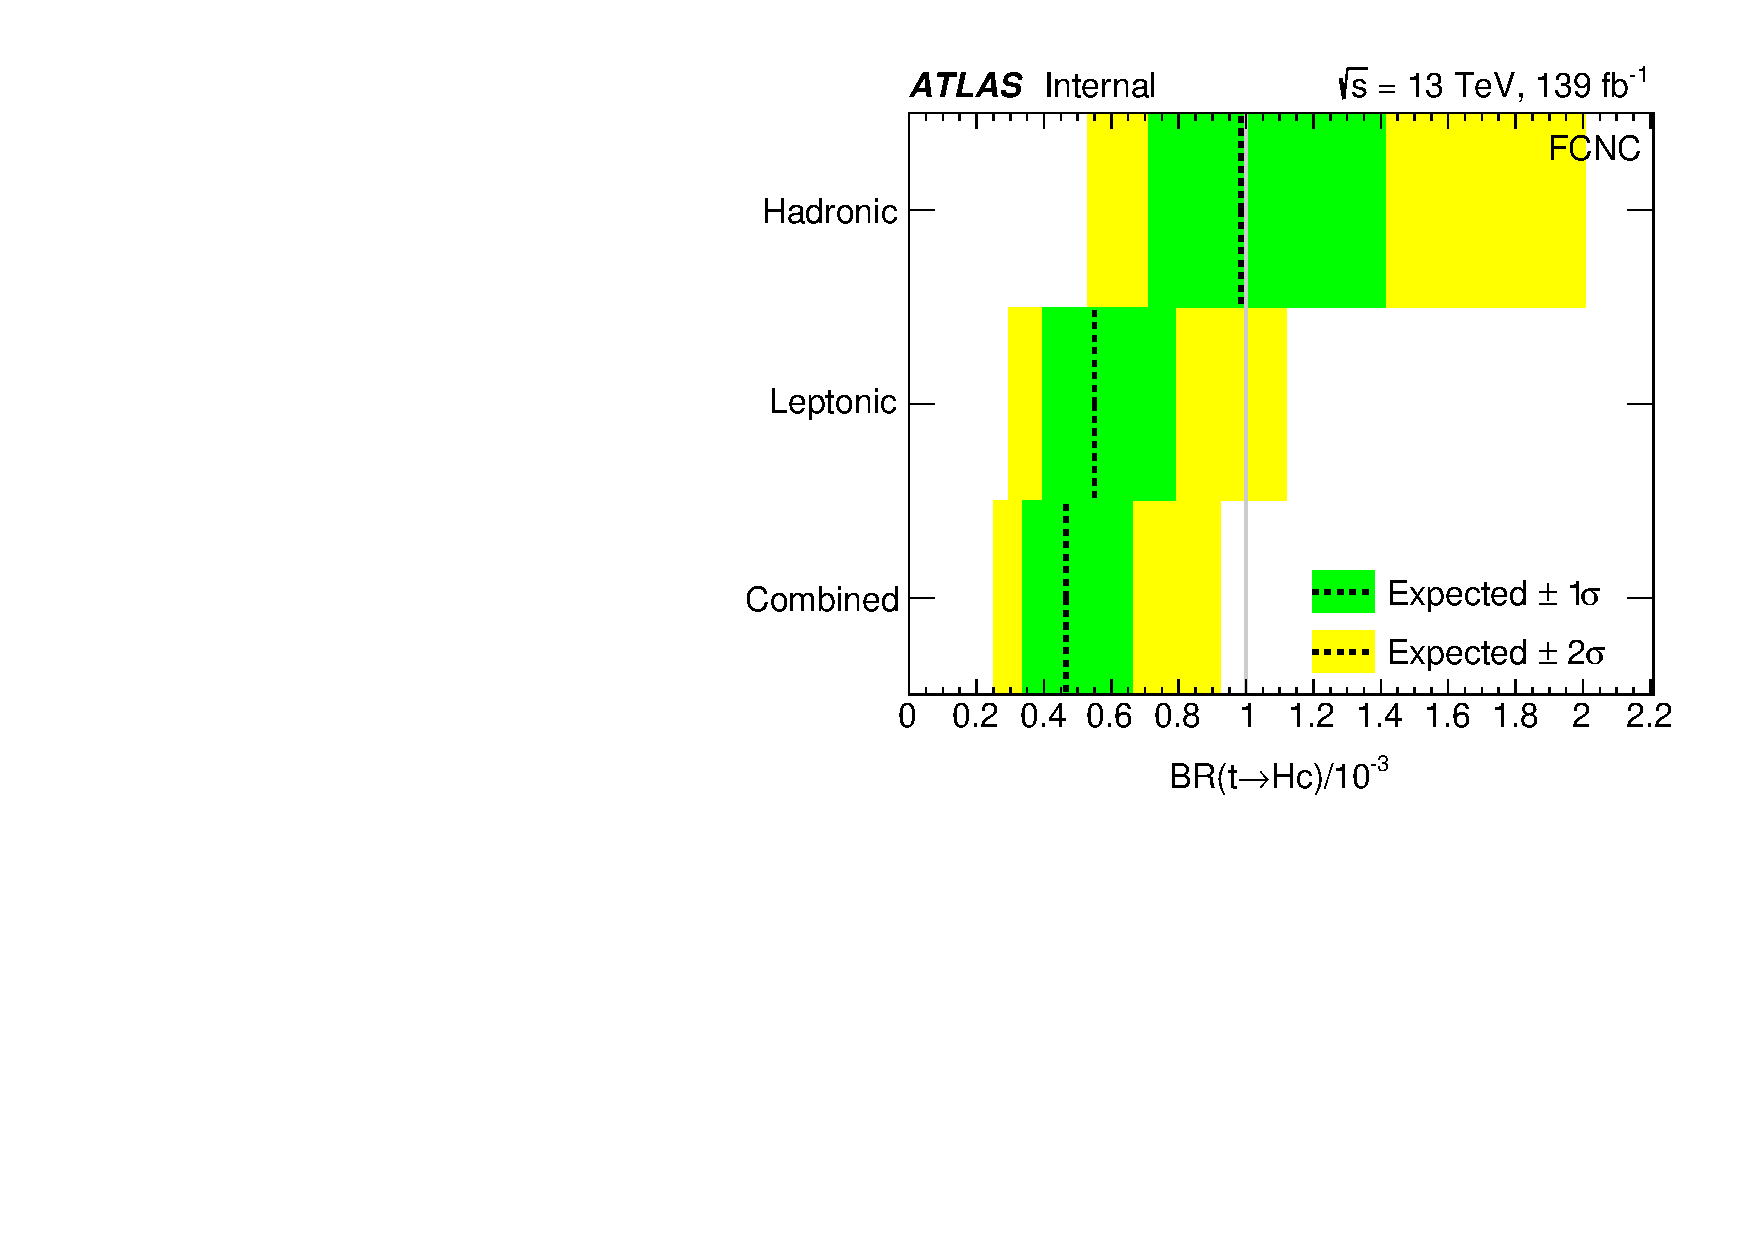
\includegraphics[width=0.7\textwidth]{\FCNCFigures/tcH_combined_Limit.pdf}
\caption{\small {95\% CL upper limits on $\BR(t\to Hc)$ for the individual searches as well as their
combination, assuming $\BR(t\to Hu)=0$. The observed limits (solid lines) are compared with the 
expected (median) limits under the background-only
hypothesis (dotted lines). The surrounding shaded bands correspond to the 68\% and 95\% CL intervals around the expected limits, 
denoted by $\pm 1\sigma$ and $\pm 2\sigma$, respectively.
}}
\label{fig:limits_combo_1D_hc} 
\end{center}
\end{figure*}
%%%%%%%%%%%%%%

%%%%%%%%%%%%%%
\begin{figure*}[h!]
\begin{center}
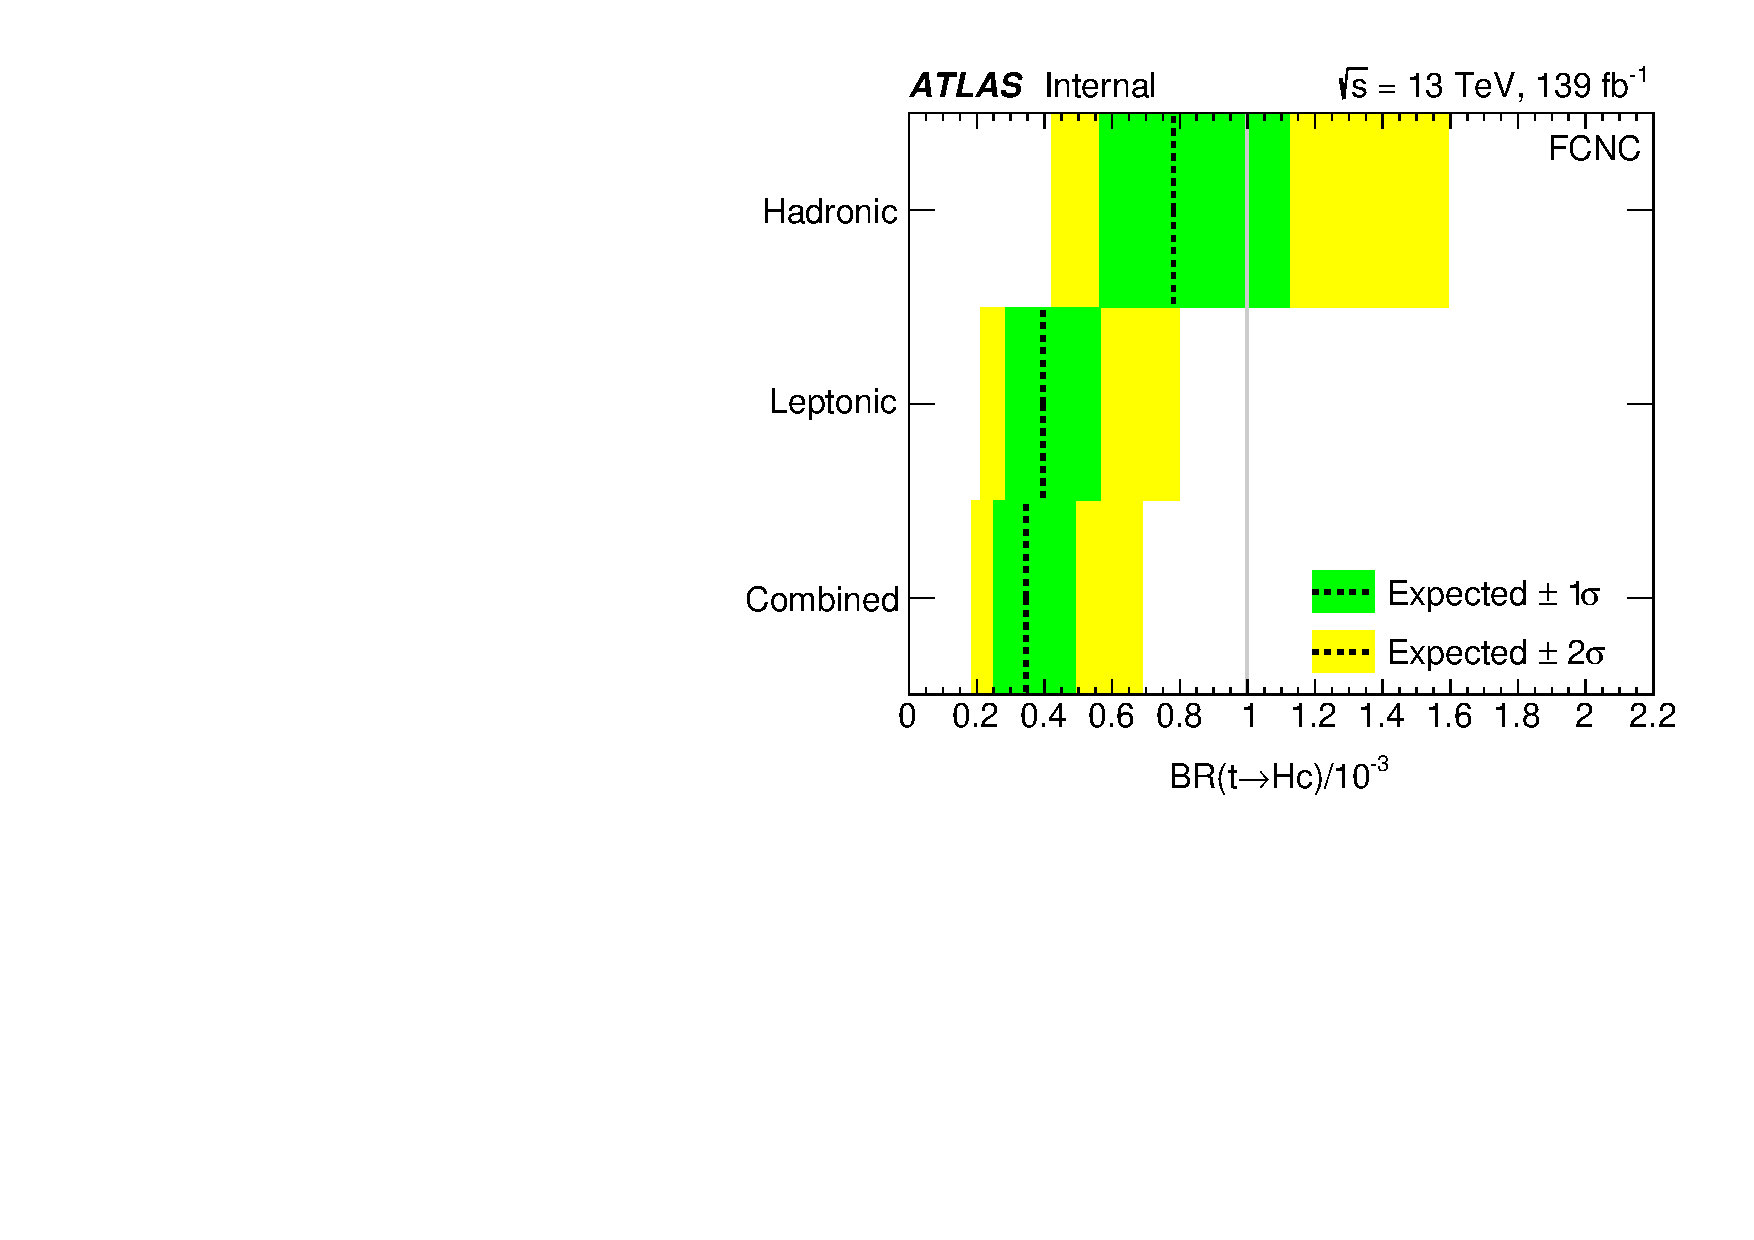
\includegraphics[width=0.7\textwidth]{\FCNCFigures/tuH_combined_Limit.pdf}
\caption{\small {95\% CL upper limits on $\BR(t\to Hu)$ for the individual searches as well as their
combination, assuming $\BR(t\to Hc)=0$. The observed limits (solid lines) are compared with the 
expected (median) limits under the background-only
hypothesis (dotted lines). The surrounding shaded bands correspond to the 68\% and 95\% CL intervals around the expected limits, 
denoted by $\pm 1\sigma$ and $\pm 2\sigma$, respectively.
}}
\label{fig:limits_combo_1D_hu} 
\end{center}
\end{figure*}

A similar set of results can be obtained by simultaneously varying both branching ratios in the likelihood function.
Figure~\ref{fig:limits_combo_2D}(a) shows the 95\% CL upper limits on the branching ratios in the $\BR(t\to Hu)$ versus $\BR(t\to Hc)$ plane. 
The small differences between the limiting values (on the $x$- and $y$-axes) of the branching ratio limits obtained in the two-dimensional scan and 
those reported in Table~\ref{tab:limits_summary}, result from slightly different choices in the $\HML$ search  
regarding the final discriminant, which in the two-dimensional case should be common to both signals, and its binning.
%\textbf{Add comment of what discriminant is used in this case and the caveat regarding the corresponding 1D limit.}
The corresponding upper limits on the couplings in the $|\lamHu|$ versus $|\lamHc|$ plane are shown in Figure~\ref{fig:limits_combo_2D}(b).

\begin{figure*}[t!]
\begin{center}
\subfloat[]{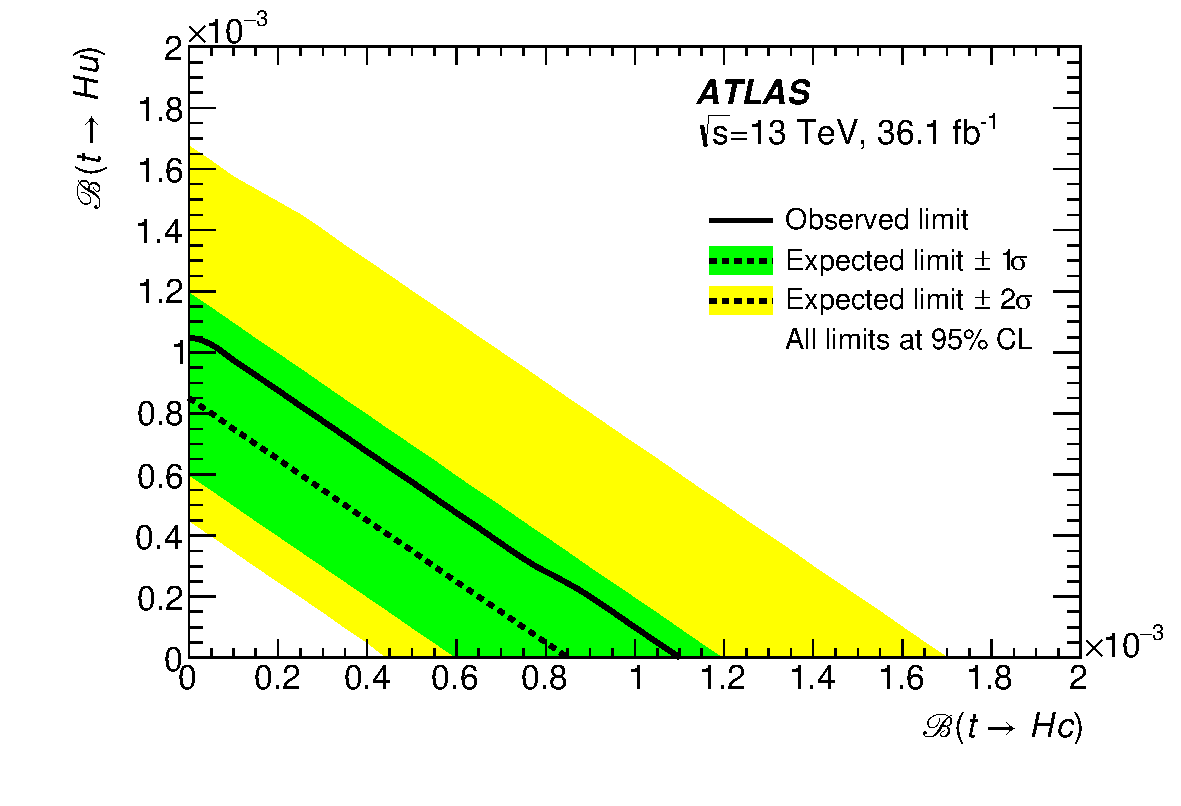
\includegraphics[width=0.49\textwidth]{figures/Combo/Limits2D.pdf}}
\subfloat[]{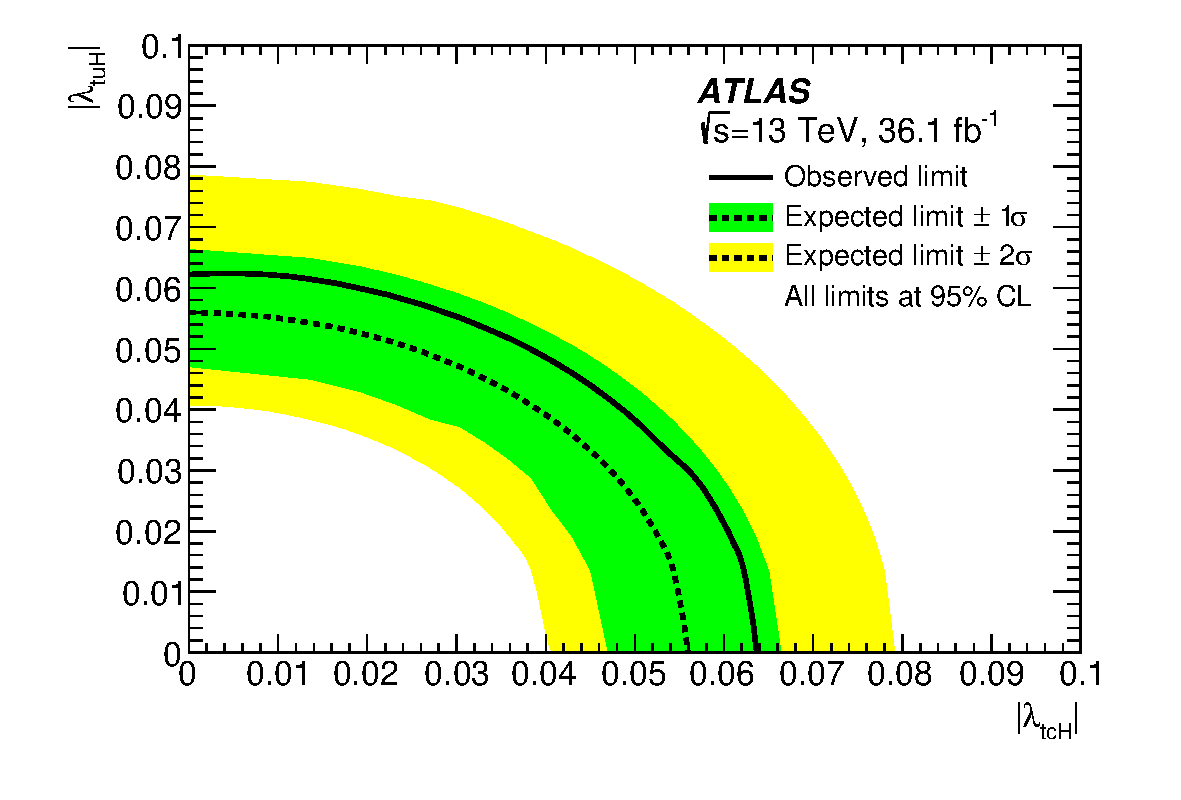
\includegraphics[width=0.49\textwidth]{figures/Combo/Coupling2D.pdf}}
\caption{\small {95\% CL upper limits (a) on the plane of $\BR(t\to Hu)$ versus $\BR(t\to Hc)$ and (b) on the plane 
of $|\lamHu|$ versus $|\lamHc|$ for the combination of the searches. The observed limits (solid lines) are compared with the expected (median) limits under the background-only hypothesis (dotted lines). The surrounding shaded bands correspond to the 68\% and 95\% CL intervals around the expected limits, 
denoted by $\pm 1\sigma$ and $\pm 2\sigma$, respectively.}}
\label{fig:limits_combo_2D} 
\end{center}
\end{figure*}
%%%%%%%%%%%%%%

